%----------------------------------------------------------------------------------------
%	PACKAGES AND OTHER DOCUMENT CONFIGURATIONS
%----------------------------------------------------------------------------------------

\documentclass{article}

%%%%%%%%%%%%%%%%%%%%%%%%%%%%%%%%%%%%%%%%%
% Lachaise Assignment
% Structure Specification File
% Version 1.0 (26/6/2018)
%
% This template originates from:
% http://www.LaTeXTemplates.com
%
% Authors:
% Marion Lachaise & François Févotte
% Vel (vel@LaTeXTemplates.com)
%
% License:
% CC BY-NC-SA 3.0 (http://creativecommons.org/licenses/by-nc-sa/3.0/)
% 
%%%%%%%%%%%%%%%%%%%%%%%%%%%%%%%%%%%%%%%%%

%----------------------------------------------------------------------------------------
%	PACKAGES AND OTHER DOCUMENT CONFIGURATIONS
%----------------------------------------------------------------------------------------

\usepackage{amsmath,amsfonts,stmaryrd,amssymb} % Math packages

\usepackage{enumerate} % Custom item numbers for enumerations

\usepackage[ruled]{algorithm2e} % Algorithms

\usepackage[framemethod=tikz]{mdframed} % Allows defining custom boxed/framed environments

\usepackage{listings} % File listings, with syntax highlighting
\lstset{
	basicstyle=\ttfamily, % Typeset listings in monospace font
}

%----------------------------------------------------------------------------------------
%	DOCUMENT MARGINS
%----------------------------------------------------------------------------------------

\usepackage{geometry} % Required for adjusting page dimensions and margins

\geometry{
	paper=a4paper, % Paper size, change to letterpaper for US letter size
	top=2.5cm, % Top margin
	bottom=3cm, % Bottom margin
	left=2.5cm, % Left margin
	right=2.5cm, % Right margin
	headheight=14pt, % Header height
	footskip=1.5cm, % Space from the bottom margin to the baseline of the footer
	headsep=1.2cm, % Space from the top margin to the baseline of the header
	%showframe, % Uncomment to show how the type block is set on the page
}

%----------------------------------------------------------------------------------------
%	FONTS
%----------------------------------------------------------------------------------------

\usepackage[utf8]{inputenc} % Required for inputting international characters
\usepackage[T1]{fontenc} % Output font encoding for international characters

\usepackage{XCharter} % Use the XCharter fonts

%----------------------------------------------------------------------------------------
%	COMMAND LINE ENVIRONMENT
%----------------------------------------------------------------------------------------

% Usage:
% \begin{commandline}
%	\begin{verbatim}
%		$ ls
%		
%		Applications	Desktop	...
%	\end{verbatim}
% \end{commandline}

\mdfdefinestyle{commandline}{
	leftmargin=10pt,
	rightmargin=10pt,
	innerleftmargin=15pt,
	middlelinecolor=black!50!white,
	middlelinewidth=2pt,
	frametitlerule=false,
	backgroundcolor=black!5!white,
	frametitle={Command Line},
	frametitlefont={\normalfont\sffamily\color{white}\hspace{-1em}},
	frametitlebackgroundcolor=black!50!white,
	nobreak,
}

% Define a custom environment for command-line snapshots
\newenvironment{commandline}{
	\medskip
	\begin{mdframed}[style=commandline]
}{
	\end{mdframed}
	\medskip
}

%----------------------------------------------------------------------------------------
%	FILE CONTENTS ENVIRONMENT
%----------------------------------------------------------------------------------------

% Usage:
% \begin{file}[optional filename, defaults to "File"]
%	File contents, for example, with a listings environment
% \end{file}

\mdfdefinestyle{file}{
	innertopmargin=1.6\baselineskip,
	innerbottommargin=0.8\baselineskip,
	topline=false, bottomline=false,
	leftline=false, rightline=false,
	leftmargin=2cm,
	rightmargin=2cm,
	singleextra={%
		\draw[fill=black!10!white](P)++(0,-1.2em)rectangle(P-|O);
		\node[anchor=north west]
		at(P-|O){\ttfamily\mdfilename};
		%
		\def\l{3em}
		\draw(O-|P)++(-\l,0)--++(\l,\l)--(P)--(P-|O)--(O)--cycle;
		\draw(O-|P)++(-\l,0)--++(0,\l)--++(\l,0);
	},
	nobreak,
}

% Define a custom environment for file contents
\newenvironment{file}[1][File]{ % Set the default filename to "File"
	\medskip
	\newcommand{\mdfilename}{#1}
	\begin{mdframed}[style=file]
}{
	\end{mdframed}
	\medskip
}

%----------------------------------------------------------------------------------------
%	NUMBERED QUESTIONS ENVIRONMENT
%----------------------------------------------------------------------------------------

% Usage:
% \begin{question}[optional title]
%	Question contents
% \end{question}

\mdfdefinestyle{question}{
	innertopmargin=1.2\baselineskip,
	innerbottommargin=0.8\baselineskip,
	roundcorner=5pt,
	nobreak,
	singleextra={%
		\draw(P-|O)node[xshift=1em,anchor=west,fill=white,draw,rounded corners=5pt]{%
		Question \theQuestion\questionTitle};
	},
}

\newcounter{Question} % Stores the current question number that gets iterated with each new question

% Define a custom environment for numbered questions
\newenvironment{question}[1][\unskip]{
	\bigskip
	\stepcounter{Question}
	\newcommand{\questionTitle}{~#1}
	\begin{mdframed}[style=question]
}{
	\end{mdframed}
	\medskip
}

%----------------------------------------------------------------------------------------
%	WARNING TEXT ENVIRONMENT
%----------------------------------------------------------------------------------------

% Usage:
% \begin{warn}[optional title, defaults to "Warning:"]
%	Contents
% \end{warn}

\mdfdefinestyle{warning}{
	topline=false, bottomline=false,
	leftline=false, rightline=false,
	nobreak,
	singleextra={%
		\draw(P-|O)++(-0.5em,0)node(tmp1){};
		\draw(P-|O)++(0.5em,0)node(tmp2){};
		\fill[black,rotate around={45:(P-|O)}](tmp1)rectangle(tmp2);
		\node at(P-|O){\color{white}\scriptsize\bf !};
		\draw[very thick](P-|O)++(0,-1em)--(O);%--(O-|P);
	}
}

% Define a custom environment for warning text
\newenvironment{warn}[1][Warning:]{ % Set the default warning to "Warning:"
	\medskip
	\begin{mdframed}[style=warning]
		\noindent{\textbf{#1}}
}{
	\end{mdframed}
}

%----------------------------------------------------------------------------------------
%	INFORMATION ENVIRONMENT
%----------------------------------------------------------------------------------------

% Usage:
% \begin{info}[optional title, defaults to "Info:"]
% 	contents
% 	\end{info}

\mdfdefinestyle{info}{%
	topline=false, bottomline=false,
	leftline=false, rightline=false,
	nobreak,
	singleextra={%
		\fill[black](P-|O)circle[radius=0.4em];
		\node at(P-|O){\color{white}\scriptsize\bf i};
		\draw[very thick](P-|O)++(0,-0.8em)--(O);%--(O-|P);
	}
}

% Define a custom environment for information
\newenvironment{info}[1][Info:]{ % Set the default title to "Info:"
	\medskip
	\begin{mdframed}[style=info]
		\noindent{\textbf{#1}}
}{
	\end{mdframed}
}
 % Include the file specifying the document structure and custom commands
\usepackage{graphicx}
\usepackage[ruled]{algorithm2e}
\usepackage{amsmath}
\SetCommentSty{mycommfont}
%----------------------------------------------------------------------------------------
%	ASSIGNMENT INFORMATION
%----------------------------------------------------------------------------------------

\title{CS221: Project Progress Report} % Title of the assignment

\author{	\textbf{Nimisha Tandon}\\  \texttt{nimisha@stanford.edu} \\
		\textbf{Shaila Balaraddi}\\  \texttt{shailaab@stanford.edu} \\
		\textbf{Naman Muley}\\      \texttt{ngmuley@stanford.edu}}

\date{\today} % University, school and/or department name(s) and a date

%----------------------------------------------------------------------------------------

\begin{document}

\maketitle % Print the title

%----------------------------------------------------------------------------------------
%	INTRODUCTION
%----------------------------------------------------------------------------------------

\section{Introduction} % Unnumbered section

We are tackling the problem of identifying articles that could be potentially dangerous to a brand. Our approach has two steps. First, we take in a set of articles and classify them into categories. In the final application, this could be done by pulling articles from the internet daily. Once these categories are identified, in the second step, we create an impact score for the brand in question. The articles with top impact scores can be provided to the client as having high potential for impact to the brand.

This problem has a rich application of various algorithms for natural language processing. Since proposing this project, we have explored a few algorithms to create a better sense of what an impact score can be. We looked into utilizing unsupervised learning algorithms like GloVe and supervised algorithm implementations like Naive Bayes. These have given us better impact scores. Further more, it feels like we could perform some more fine tuning to come up with better models to bring a richer understanding of the \textit{impact score}

\maketitle % Print the title
%----------------------------------------------------------------------------------------
%	MODEL
%----------------------------------------------------------------------------------------
\section{Methodology} % Unnumbered section
We extend our two step approach which we presented in the proposal. We have spent time exploring different algorithms for both these stages. We seem to have settled on to a methodology, which we explain in this section.

\subsection {Classification}
In making progress for the project, we decided to give more weight to the impact score analysis section, since that's the more novel component of the solution approach. Our classification currently still uses a simple Stochastic Gradient Descent classifier. We found it's accuracy to be nearly 82 percent and thought we can improve upon that in the later parts of the project.

We still did look at using the Naive Bayes algorithm to perform classification, since that's what literature reported is it's primary use. It performed slightly better at classification than SGD but not by much.

\subsection {Impact Score}

Impact score needs to be a number that represents how relevant or impactful will a particular article be to the brand. Hence, we extended our previous approach of having a vocabulary of words that are relevant to the brand and applying a combination GloVe analysis, TF-IDF and Naive Bayes to come up with a score of how closely does the article's content relate to the dictionary relevant to the brand.

\subsubsection {Input Brand Vocabulary}
It was possible to decipher a set of words that are deemed contextually more dominant and important for a category like \textit{guns} by various methodologies including TF-IDF itself. But we believe finding relevancy to a brand should allow some input bias from the brand. For example, a brand may way to find articles relevant to a subset of their very specific products and those may not be popularly present in the testing dataset.

We allow a list of words to act as our vocabulary for finding articles with highest potential impact. For example, for a brand like NRA, we take the following set of words as a vocabulary:
\begin{center}
["guns", "shooting", "weapon", "nra", "handgun", "assault", "rifle", "america", "firearm"]
\end {center}

\subsubsection {Similar Words using GloVe learning}
A measure of how relevant an article is to a brand is to know how many of semantically or linguistically similar words occur in that article. For each of the words in the vocabulary, we get a list of \textit{similar words} using the GloVe learning algorithm [1]. We then use a simple TF algorithm to understand how commonly do these similar words occur in an article.

\begin{center}
\begin{algorithm}
  \caption{Extend Vocabulary with Similar Words using Glove Model}
  \SetKwInOut{Input}{inputs}
  \SetKwInOut{Output}{output}
  \SetKwProg{GetGloveWords}{GetGloveWords}{}{}

 $Vocabulary \gets ["guns", "rifle", "weapon", "nra", "handgun", "firearm"] $\;
 $model \gets train\_glove(\textit{glove.6B.300d.w2vformat.tx}) $\;
 \GetGloveWords{$(Vocabulary, model)$} {
      $extended\_vocab \gets Vocabulary $\;
     \ForEach{word $w \in Vocabulary$}{%
       $similar\_words \gets model.get\_similar\_words($word=w, $topN=10) $\;
       $extended\_vocab.extend($similar\_words$) $\;
      }
    \KwRet{$extended\_vocab$}\;
  }
\end{algorithm}
\end{center}

Once the vocabulary is extended, we use this extended vocabulary to identify articles that have the most occurrences of these words. In the Proposal, we had used a similar algorithm to calculate our baseline but with the vocabulary as the raw input set of words. Following is a figure that shows how the expanded vocabulary behaves for a brand like NRA and input vocabulary = \textit {["guns", "weapons", "nra"]}.

\begin{figure}[ht]
	\centering
 	 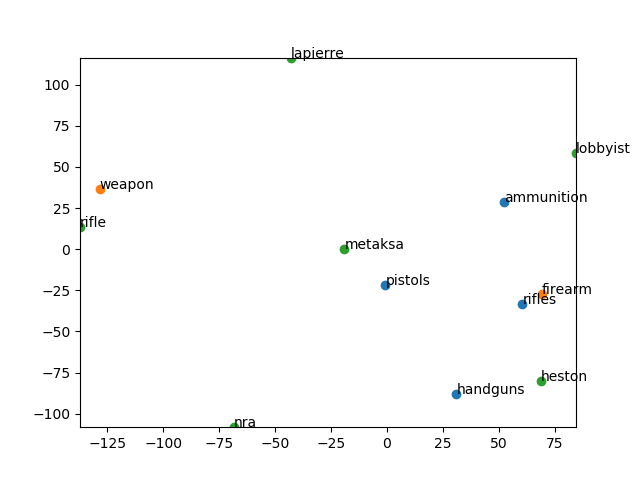
\includegraphics[width=0.5\linewidth]{similar_words_nra.png}
	  \caption{Similar Words obtained from GloVe Learning for \textit{NRA}}
 	 \label{fig:Similar Words for NRA}
\end{figure}

We use this extended vocabulary to come up with an impact score by simply counting frequencies of these words. Our algorithm that performs this to come up with an impact score for each article in the category is given below. The score dictionary contains the impact score calculated for each article in the set of articles.

\begin {center}
\begin {algorithm}[ht]
\SetNoFillComment
\caption{Calculate Impact Score for each article from a list of articles, given extended vocabulary}
\SetKwInOut{Input}{inputs}
\SetKwInOut{Output}{output}
\SetKwProg{CalculateVocabImpactScore}{CalculateVocabImpactScore}{}{}
\CalculateVocabImpactScore{$(V, D)$} {
    \Input{A list of words that form ExtendedVocabulary V; a list of articles D}
    \Output{A dictionary representing impact scores for all articles in D}
    $score \gets \emptyset $\;
    $RangeD \gets range(0, len(D)) $\;
    \ForEach {index $i \in RangeD$} {
    	score[i] = 0 \;
	freq = [] \;
	\tcc{iterate over all words in $i_{th}$ article to count frequency}
	\ForEach {word $w \in D[i]$} {
		freq[word] += 1 \;
	}
	\tcc{iterate over all words in V to build a score for article $i$}
	\ForEach {word $w \in V$} {
		score[i] += freq[w] \;
	}
    }
    score.Normalize() \;
    \KwRet{$score$}\;
}
\end {algorithm}
\end {center}

We have detailed our results of the above score dictionary in the Results section.

\subsubsection {Relevant words using TF-IDF}

Term Frequency-Inverse Document Frequency commonly known as TF-IDF can be used to find the frequency of vocabulary words in a document to perform sentiment analysis or extract relevancy from a document.

This algorihm has 2 algorithms working together.
\begin{enumerate}
\item {Term Frequency}
\[tf(t,d) =  = \frac{no of occurrences of term in doc }{total number of all words in document}\]


Before using this algorithm, we first do some preprocessing of the doc as follows:
\begin{itemize}
\item {Remove all stop words.(ex: in, the,are it)}
\item {Convert all words to lowercase.}
\end {itemize}
Now using the term frequency alone will end up giving us words that are not unique (for ex: repeated words, should not add up to the relevance of the document)

\item Inverse document frequency

 This gives us the uniqueness of a word:

 \[idf(t,d) =  = log(\frac{no of times the term appears }{no of documents containing the word})\]

The final step is to multiply the two together to get the TFIDF score which would give us the impact score.
\end{enumerate}


\maketitle
%---------i-------------------------------------------------------------------------------
%	IMPLEMENTATION
%----------------------------------------------------------------------------------------
\section{Implementation} % Unnumbered section
Following are some important points to mention about implementation details:
\begin {itemize}
\item \textit{Application} Currently we have a python application that performs the training of the supervised algorithms and data transformations. We are working on a single \textit {guns} category. We also use a static set of vocabulary mentioned above, assuming we got that as input from a fictitious National Rifles Association (NRA) client
\item \textit {GloVe training} GloVe has been trained on the \textit{Wikipedia 2014 + Gigaword 5} dataset mentioned on the project's website (\textit{https://nlp.stanford.edu/projects/glove/})
\item \textit {Compute} We noticed that running GloVe on a laptop is not fast. Going forward we will use the compute credits provided to us.
\end {itemize}

 \maketitle
%----------------------------------------------------------------------------------------
%	PRELIMINARY RESULTS
%----------------------------------------------------------------------------------------
\section{Preliminary Results} % Unnumbered section
We will outline the impact scores we identified using both the methods below. We are yet to come up with a justifiable way to combine these scores to present a single final score:
We ran the above algorithms and ran comparisons on various impact score results on the documents.
We tried two different approaches and got different yet comparable results.

Another observation is that the old scores seem higher than the new ones. This is because of the naive approach in the baseline program, that ran frequency check on documents without any pre-processing or vocabulary extensions. As can be seen in the appendix, the latest results are more relevant to the subject of "guns".

\subsection{Extracting vocabulary using Glove}
Ran a Glove vocabulary extension to add to the limited vocabulary we had earlier. This definitely helped pull more relevant documents to the front.
If we compare the results with the impact scores presented in the Proposal, we notice that articles have shuffled up a bit. Here are some points to consider:
\begin {enumerate}
\item Article index 7274 was at the top, now it is in 4th place, whereas 5893 is at the top now.
\item Article 5893 is a long article about 2nd ammendment, which is extremely relevant to NRA while 7274 is an article about gun buy backs, which is also fairly relevant.
\item Article 2135 has remained at the 10th place.
\end {enumerate}

\begin{table}[ht]
\caption{Impact Score chart} % title of Table
\centering % used for centering table
\begin{tabular}{|p{3cm}|p{3cm}|p{3cm}| } % centered columns (4 columns)
\hline\hline %inserts double horizontal lines
DocId & Old Score & New Score\ \\ [0.5ex] % inserts table
%heading
\hline % inserts single horizontal line
5893 & 0
  & 0.021 \\ % inserting body of the table
  692 & 0
  & 0.017 \\ % inserting body of the table
  6763 & 0.02
  & 0.016 \\ % inserting body of the table
  7274 & 0.05
  & 0.014 \\ % inserting body of the table
  326 & 0.05
  & 0.014 \\ % inserting body of the table
    3613 & 0.03
  & 0.014 \\ % inserting body of the table
    3831 & 0
  & 0.013 \\ % inserting body of the table
    1665 & 0.02
  & 0.011 \\ % inserting body of the table
    3781 & 0.01
  & 0.011 \\ % inserting body of the table
    2135 & 0.01
  & 0.010 \\  [1ex] % [1ex] adds vertical space
\hline %inserts single line
\end{tabular}
\label{table:nonlin} % is used to refer this table in the text
\end{table}

\subsection{Using term frequency(TF) on classified documents}
We added a new method of classification using Naive Bayes classifier to classify the documents into categories.
The impact score was going through pre-classified documents. Ran the documents through a cleanup and then calculated term-frequency of the vocab words to get the impact score.
Observed that the results did bring some previously unseen relevant documents to the front. Specifically the smaller documents that were dense on the subject(vocab words).
\begin{table}[ht]
\caption{Impact Score chart} % title of Table
\centering % used for centering table
\begin{tabular}{|p{3cm}|p{3cm}|p{3cm}| } % centered columns (4 columns)
\hline\hline %inserts double horizontal lines
DocId & Old Score & New Score\ \\ [0.5ex] % inserts table
%heading
\hline % inserts single horizontal line
7417 & 0
  & 0.020 \\ % inserting body of the table
  1844 & 0.05
  & 0.019 \\ % inserting body of the table
  6620 & 0
  & 0.018 \\ % inserting body of the table
  548 & 0.03
  & 0.017 \\ % inserting body of the table
  7274 & 0.05
  & 0.015 \\ % inserting body of the table
    6896 & 0
  & 0.015 \\ % inserting body of the table
    1902 & 0
  & 0.015 \\ % inserting body of the table
    3725 & 0
  & 0.015 \\ % inserting body of the table
    3104 & 0
  & 0.014 \\ % inserting body of the table
    2668 & 0.03
  & 0.014 \\  [1ex] % [1ex] adds vertical space
\hline %inserts single line
\end{tabular}
\label{table:nonlin} % is used to refer this table in the text
\end{table}


\maketitle
%----------------------------------------------------------------------------------------
%	FUTURE WORK
%----------------------------------------------------------------------------------------
\section {Future Work}
This impact score, we feel, still does not capture all the richness we can provide using natural language processing algorithms. We intend to improve in the following areas:
\begin {enumerate}
\item \textit {Combining Scores from Different algorithms}: TF-IDF and GloVe, both gave a varying set of articles that each thought were more impactful. We would like to investigate good strategies to combine these and present a final score.
\item \textit {Aspect based Sentiment Analysis}: ABSA is another methodology that literature showed is a good way of identifying important articles. Add aspect based sentiment analysis where we will come up with some aspects which add more meaning to the impact score.
\item \textit {Expand the number of categories}: Generalizing our work to focus on more categories
\item \textit {Better Trained Models}: Currently the GloVe model we use is trained from the wikipedia dataset. We intend to see if training it on a more relevant dataset creates a better set of similar words that we can use to calculate impact scores
\end {enumerate}


\maketitle
%----------------------------------------------------------------------------------------
%	APPENDIX
%----------------------------------------------------------------------------------------
\section {Appendix}
Top relevant documents for "guns"

\item
id: 5893

Subject: Analysis of Second Amendment (Was: Re: Some more about gun control...)
Organization: Totally Unorganized
Lines: 267

In article <1993Apr21.042608.26086@ra.msstate.edu> dnewcomb@whale.st.usm.edu (Donald R. Newcomb) writes:
>First, I would like to say how much I appreciate having so literate and
>erudite an individual as Mr. Rutledge with whom to discuss this topic.
>Frankly, most anti-RKBA posters refuse even to approach the topic of
>the original understanding of the Bill of Rights as detailed in the
>writings of the era. This  is most refreshing.
>
>Second, I must apologize for leaving the discussion for several days.
>My brigade's quarterly drill was this weekend and I needed to attend
>to several matters pertaining to the State Militia.
>
>Some people seem to feel that the concept of the Militia is an anachro-
>nism that is out of place in the 20th century. I'm not sure the Swiss
>would agree and I think perhaps a discussion of how the Militia, both
>organized and unorganized, fits into the defense plans of my State,
>Mississippi. Please do not assume that this describes something peculiar
>to one southern state. For instance, the Commonwealth of Massachusetts
>has a well organized Militia which, members report, maintains stocks
>of both riot guns and machine guns. The laws of other States will vary
>but are probably similar.

It appears it is time that this article (originally posted by Larry
Cipriani last year, and which I saved) gets posted again.  It offers
as good an analysis of the meaning of the Second Amendment, especially
regarding the militia clause, as I have seen.  I have not seen any
rebuttles with similar bone fides...

Enjoy.  (Flames to /dev/null)

--------- Begin Enclosed Article -----------

                        THE UNABRIDGED SECOND AMENDMENT

                              by J. Neil Schulman

If you wanted to know all about the Big Bang, you'd ring up Carl Sagan,
right ?  And if you wanted to know about desert warfare, the man to call
would be Norman Schwarzkopf, no question about it.  But who would you call
if you wanted the top expert on American usage, to tell you the meaning
of the Second Amendment to the United States Constitution ?

That was the question I asked A.C. Brocki, editorial coordinator of the Los
Angeles Unified School District and formerly senior editor at Houghton
Mifflin Publishers -- who himself had been recommended to me as the
foremost expert on English usage in the Los Angeles school system.  Mr.
Brocki told me to get in touch with Roy Copperud, a retired professor
journalism at the University of Southern California and the author of
"American Usage and Style: The Consensus."

A little research lent support to Brocki's opinion of Professor Copperud's
expertise.

\item
Id: 7274

Subject: Re: Gun Buy Back
From: R1328@vmcms.csuohio.edu
Organization: CSU
Lines: 150

In article <1r6qqcINN8j4@clem.handheld.com>
jmd@cube.handheld.com (Jim De Arras) writes:

>
>In article <16BB8B194.R1328@vmcms.csuohio.edu> R1328@vmcms.csuohio.edu writes:
>> In article <1993Apr22.134330.9761@rti.rti.org>
>> jbs@rti.rti.org writes:
>>
>> >
>> >In article <16BB7BA6A.R1328@vmcms.csuohio.edu> R1328@vmcms.csuohio.edu
>writes:
>> >>...Gun buyback programs will hopefully
>> >>have an impact on accidental shootings (especially youths), domestic
>> >>disputes where a gun is available in the heat of emotion and anger, and
>> >>maybe keep a few guns from being stolen and later used in street-level
>> >>crime.
>> >
>> >What gives you the idea that gun "buyback" programs will have an impact on
>> >any of these things?  Evidence, please?
>> >
>> > Please don't misinterret  what I was saying Joe.  I was making the point
>tha
>> there is NO evidence of effect of gun buyback programs but hopefully if
>> there is any effect it may prevent injuries or deaths in one of these types
>> of common incidents.
>>
>> >If you're a "Research Associate" in "Urban Child Research," then perhaps
>> >you can comment for us on the ratio of the accidental gun death rate to the
>> >rate of accidental death from other single causes?  Follow that perhaps
>> >with some sort of justification for the amount of effort that anti-gunners
>> >spend trying to convince the country that accidental gun-related death
>> >among children in the U.S. is a serious problem.
>> >
>>  Firearms are the fifth-leading cause of unintentional deaths among children
>> ages 14 and under.  I don't understand how the ratio to other accidental
>> deaths is important.  So guns don't kill as many children as car accidents.
>> What is the difference in severity between 1,000 deaths and 10,000 deaths?
>> I am not trying to use accidental gun-related deaths among children as a
>> justification for gun control.  Who needs to be convinced that accidental
>> gun deaths of children is a serious problem?  I assumed that any humane
>> person would be concerned when any 10 year old got hold of their parents
>> gun from their bedroom drawer and accidently blew away one of their friends.
>>

\item
Id:6620

From: alane@microsoft.com (Alan Ezekiel)
Subject: Re: The Dayton Gun "Buy Back" (Re: Boston Gun Buy Back)
Organization: Microsoft Corporation
Lines: 63

>lvc@cbnews.cb.att.com (Larry Cipriani) writes:
>
>>According to WNCI 97.9 FM radio this morning, Dayton, Ohio is operating a
>>gun "buy back".  They are giving $50 for every functional gun turned in.
>>They ran out of money in one day, and are now passing out $50 vouchers of
>>some sort.  They are looking for more funds to keep operating.  Another
>>media-event brought to you by HCI.
>>
>>Is there something similar pro-gun people can do ?  For example, pay $100
>>to anyone who lawfully protects their life with a firearm ?  Sounds a bit
>>tacky, but hey, whatever works.

As David Veal points out, this sort of "promotion" would be used
against gun owners by the mass media.

However, here is my proposal: offer gun safety classes in your area,
free, as a community service.  Such a class would normally cost $40
or $50, so offering it free is a good promotion.

Our Gun Club has organized several of these (we just finished
teaching another one last night, in fact) and they have been
very well received.  We get a lot of people who are novices
interested in guns.  We even get a few who are anti-gun, but
feel they should know something about "gun safety" since members
of their family keep guns at home.

Teaching such a course gives us many desirable benefits:

(1) We have the chance to teach gun safety rules; this increases
    firearm awareness and may help to reduce gun accident stats.

(2) A "gun safety" class is Politically Correct, and likely to
    be viewed positively by the public and the media.

(3) Most of the students are 'normal people' (not gun enthusiasts)
    and this kind of class gives us the chance to give them a
    gentle introduction to firearms.

(4) Some of the students are enthusiastic, and will purchase a gun
    and become more involved in shooting or personal defense.

(5) It improves the public perception of our club and gun owners
    in general.  Our students see that we are all reasonable,
    non-aggressive, soft-spoken people, which helps to mitigate
    the standard image of a hardcore gun owner.  Even anti-gun
    students sometimes tell us they have "something new to think
    about" with regards to personal gun ownership.

(6) Sharing our experience with others is a lot of fun.

Our course is the standard NRA-certified "Home Firearm Safety"
class, and our students pay only $5 for materials.  We also
teach the NRA's "Personal Protection" class, although the cost
is higher for that one since we have to purchase range time.

I think firearms safety classes are an excellent response to
gun buy-backs.


\end{document}